\section*{Ordenação}

\begin{frame}
	\begin{block}{Técnicas de Ordenação}
		\begin{itemize}
			\item Ordenação é uma atividade frequente ao programar
			
			\item Os algoritmos usam estratégias de ordenação variadas que mostram diversas técnicas de programação
		\end{itemize}
	\end{block}
\end{frame}


\begin{frame}
	\begin{block}{InsertionSort}
		\begin{itemize}
			\item Vamos começar pelo algoritmo de ordenação: "insertionSort", a estratégia de ordenação é baseada em ordenar uma "mão de cartas". 

			\item Onde o jogador colocar uma a uma as menores cartas na esquerda até que a mão toda fique ordenada.
		\end{itemize}
	\end{block}
\end{frame}

\begin{frame}	
	\begin{block}{}	
		 \begin{figure}[!htb]
			\centering	  				
			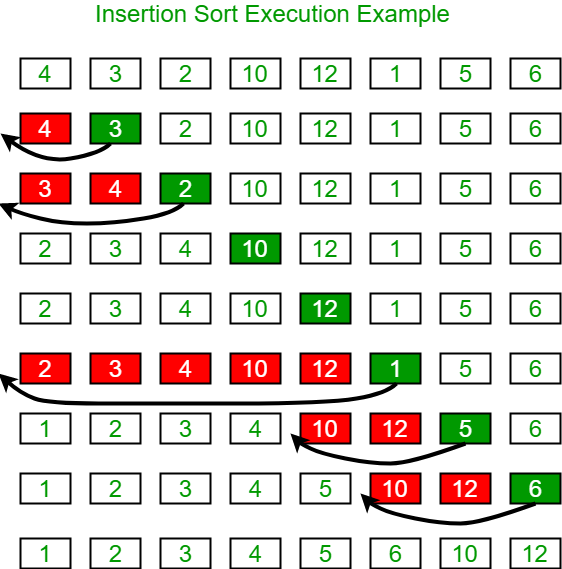
\includegraphics[height=5cm, width = 9cm]{./pic/insertionsort.png}
			\caption{Exemplo de execução do Insertion Sort}
			\label{fig_analise_insertion}
		\end{figure}
	\end{block}
\end{frame}

\begin{frame}
	\begin{block}{InsertionSort}
		\begin{itemize}
			\item Programar com os alunos
			\item Mostrar complexidade
		\end{itemize}
	\end{block}
\end{frame}


\begin{frame}{}
	\begin{figure}[h!]
		\centering    
		\movie[
					   height = 6cm,%
		                width = 6cm,%
		                %poster,
		                showcontrols%
					] 
		  {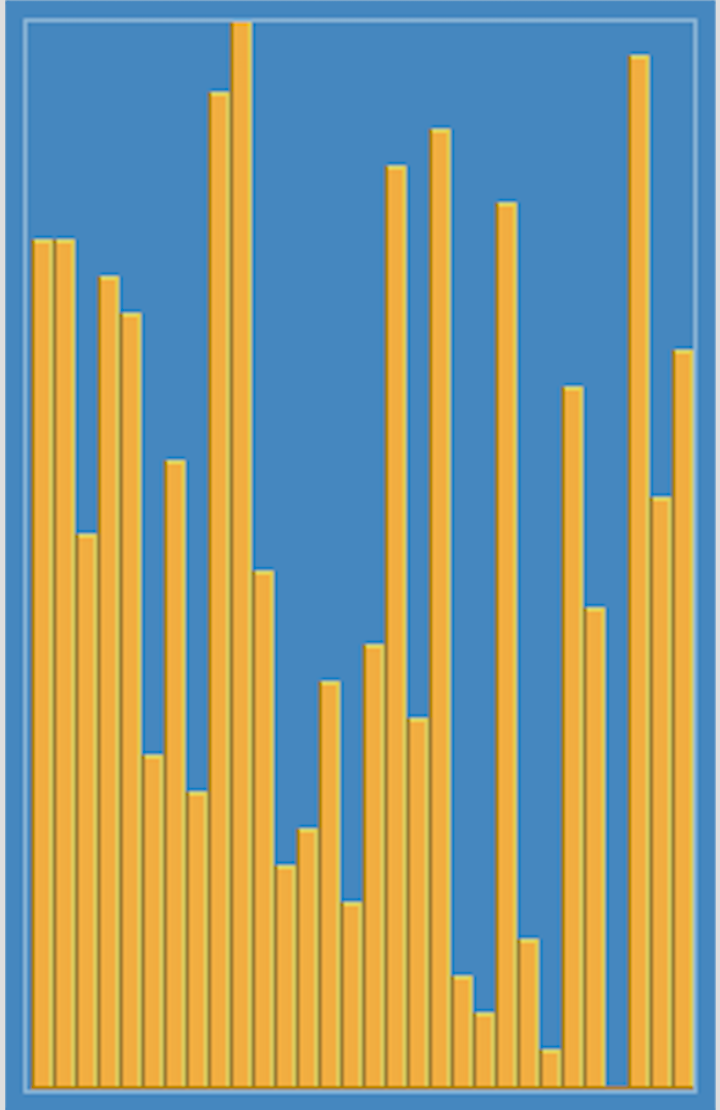
\includegraphics[width=5cm, height = 6cm]{./pic/IS_poster.png}}{./pic/Insertion_sort.mov}
		  \caption{Exemplo de ordenação com o Insertion Sort}
	 \end{figure} 
\end{frame}

\begin{frame}
	\begin{block}{BubbleSort}
		\begin{itemize}
			\item Este algoritmo pega cada elemento e troca com o seguinte, contanto que o seguinte seja maior, até o ponto onde não ocorre mais troca. Em seguida, pega o segundo elemento no vetor até acabarem os elementos nos vetores.
		\end{itemize}
	\end{block}
\end{frame}

\begin{frame}
	\begin{block}{BubbleSort}
		\begin{itemize}
			\item Programar com os alunos
			\item Mostrar complexidade
		\end{itemize}
	\end{block}
\end{frame}

\begin{frame}{}
	\begin{figure}[h!]
		\centering    
		\movie[
					   height = 6cm,%
		                width = 6cm,%
		                %poster,
		                showcontrols%
					] 
		  {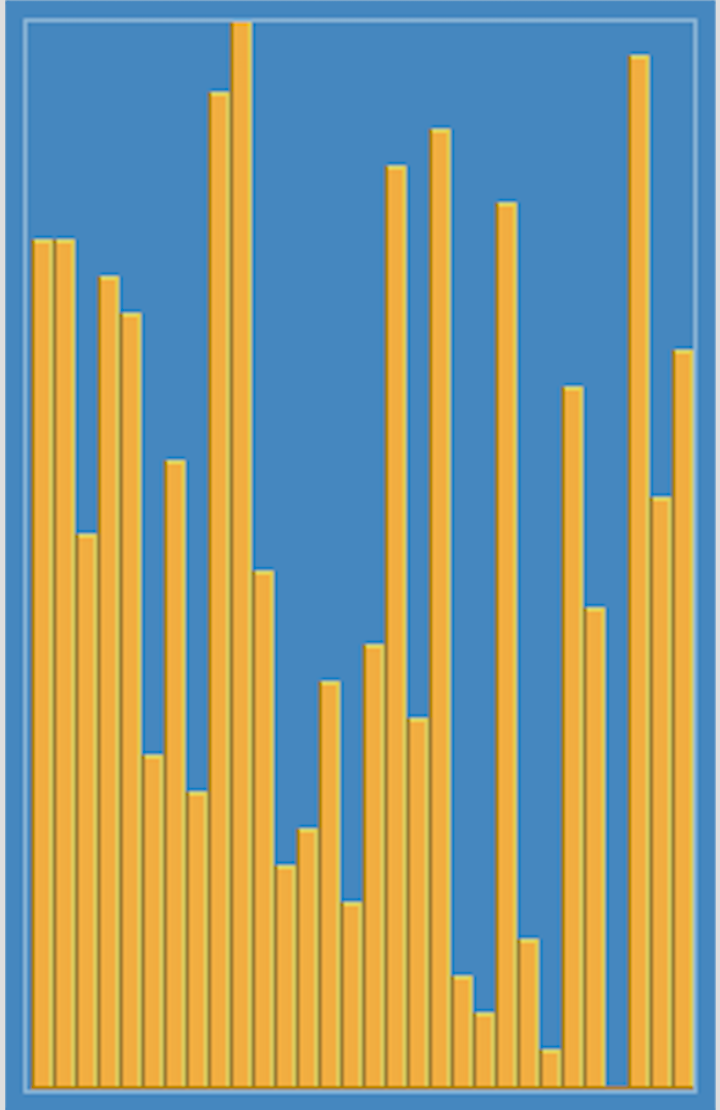
\includegraphics[width=5cm, height = 6cm]{./pic/IS_poster.png}}{./pic/bubleSort.mov}
		  \caption{Exemplo de ordenação com o BubbleSort}
	 \end{figure} 
\end{frame}

\begin{frame}
	\begin{block}{MergeSort}
		\begin{itemize}
			\item Particiona o vetor de dois em dois até que só tenha um elemento de forma recursiva. Volta fazendo uma fusão com ordenação dos dois elementos, em seguida, faça a fusão com as outras partes duas a duas até juntar novamente o vetor único e ordenado
		\end{itemize}
	\end{block}
\end{frame}

\begin{frame}	
	\begin{block}{}	
		 \begin{figure}[!htb]
			\centering	  				
			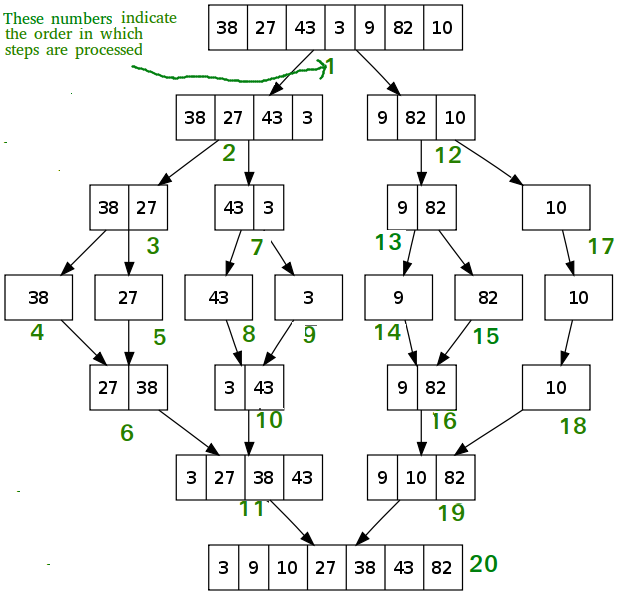
\includegraphics[height=5cm, width = 9cm]{./pic/Merge-Sort-Tutorial.png}
			\caption{Merge Sort}
			\label{fig_merge}
		\end{figure}
	\end{block}
\end{frame}

\begin{frame}{}
	\begin{figure}[h!]
		\centering    
		\movie[
					   height = 6cm,%
		                width = 6cm,%
		                %poster,
		                showcontrols%
					] 
		  {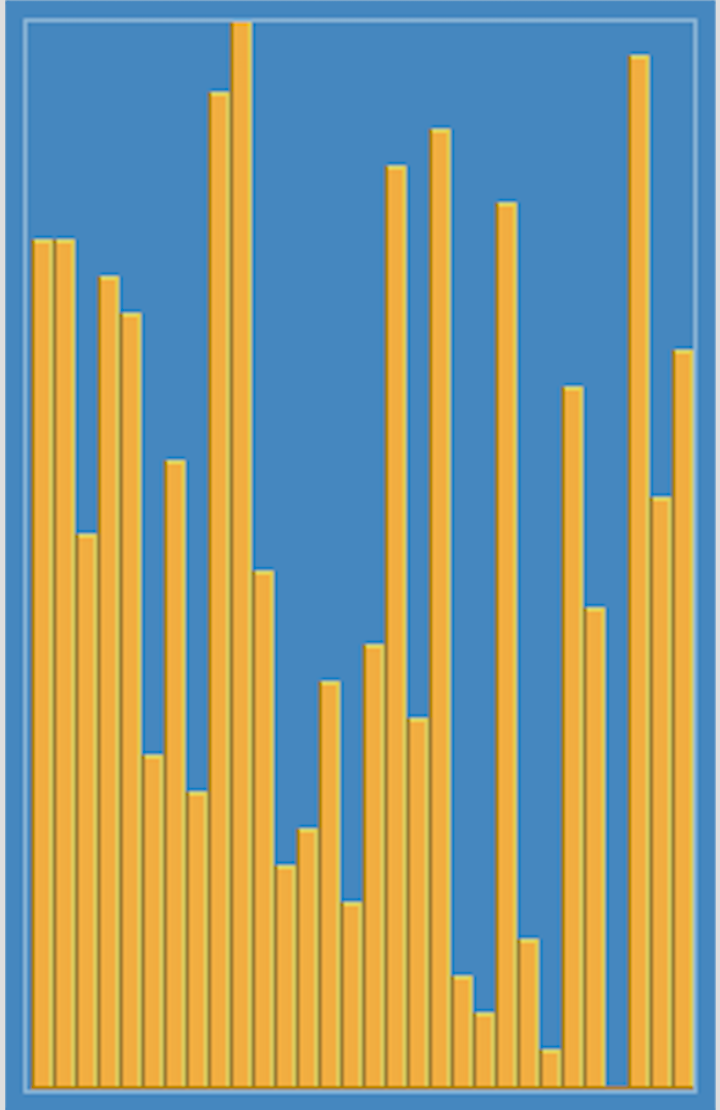
\includegraphics[width=5cm, height = 6cm]{./pic/IS_poster.png}}{./pic/mergeSort.mov}
		  \caption{Exemplo de ordenação com o MergeSort}
	 \end{figure} 
\end{frame}

\begin{frame}
	\begin{block}{MergeSort}
		\begin{itemize}
			\item Programar com os alunos
			\item Mostrar complexidade
		\end{itemize}
	\end{block}
\end{frame}


\begin{frame}
	\begin{block}{QuickSort}
		\begin{itemize}
			\item Escolhe um pivô no vetor, separa os outros elementos em maiores e menores ou iguais ao pivô. Para cada subconjunto criado (maiores e menores) encontre um novo pivô e repita o procedimento de forma recursiva.até que as partições sejam vazias. Ao terminar, o array já está ordenado pois o próprio array foi usado para armazenar as partições.
		\end{itemize}
	\end{block}
\end{frame}


\begin{frame}	
	\begin{block}{}	
		 \begin{figure}[!htb]
			\centering	  				
			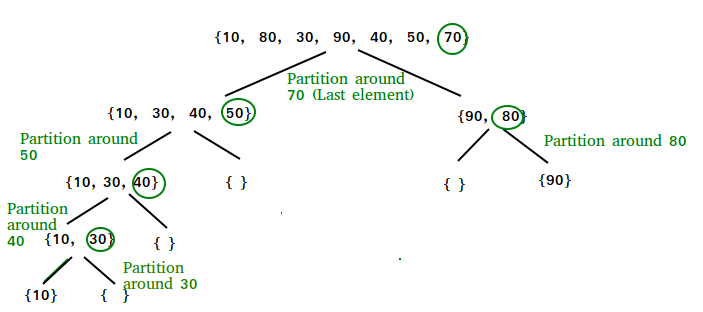
\includegraphics[height=5cm, width = 9cm]{./pic/QuickSort2.png}
			\caption{QuickSort}
			\label{fig_merge}
		\end{figure}
	\end{block}
\end{frame}

\begin{frame}{}
	\begin{figure}[h!]
		\centering    
		\movie[
					   height = 6cm,%
		                width = 6cm,%
		                %poster,
		                showcontrols%
					] 
		  {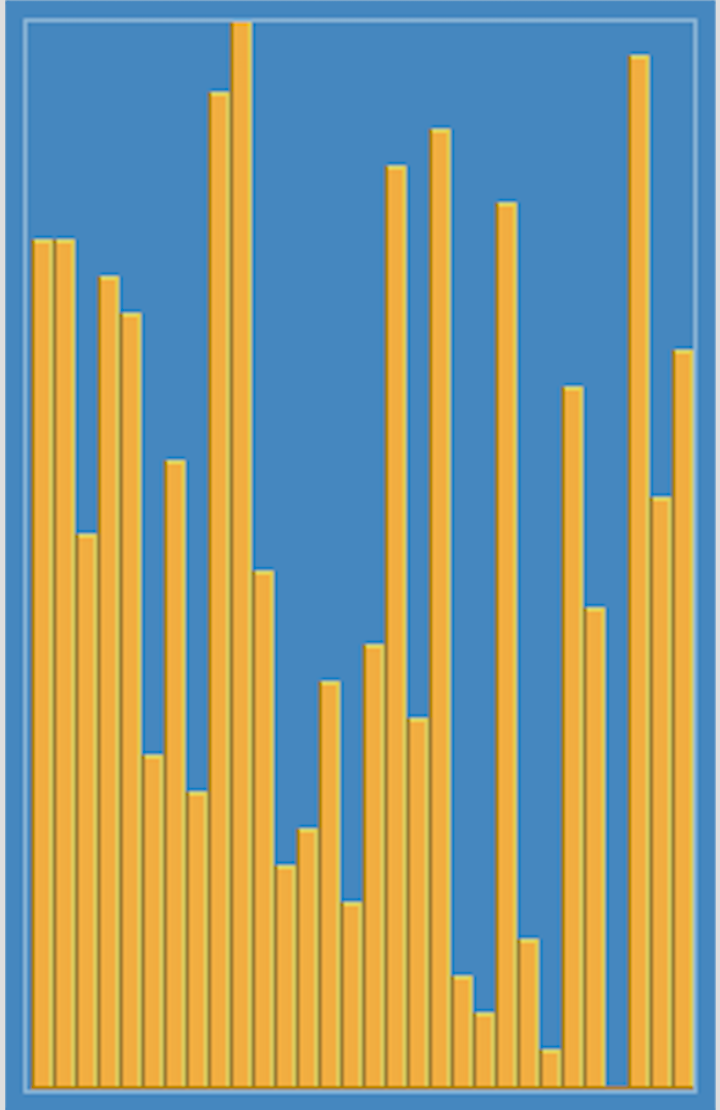
\includegraphics[width=5cm, height = 6cm]{./pic/IS_poster.png}}{./pic/quickSort.mov}
		  \caption{Exemplo de ordenação com o QuickSort}
	 \end{figure} 
\end{frame}

\begin{frame}
	\begin{block}{QuickSort}
		\begin{itemize}
			\item Programar com os alunos
			\item Mostrar complexidade
		\end{itemize}
	\end{block}
\end{frame}

